\documentclass[conference]{IEEEtran}
\IEEEoverridecommandlockouts

\usepackage{cite}
\usepackage{amsmath,amssymb,amsfonts}
\usepackage{graphicx}
\usepackage{xcolor}
\usepackage{url}
\usepackage{hyperref}
\usepackage{booktabs}
\usepackage{siunitx}
\usepackage{comment}

\newcommand{\tcite}{\textbf{[@TODO]}}

\begin{document}

\title{AsimovBM: Toward Automatic Evaluation of\\
Human-Perceived Traits in Physical AI 
Robots
% Robotics Agents
}

\author{
  \IEEEauthorblockN{Andrea Tosi, Niccolò Dellepiane, Luis Sebastian Caballero Fritas,
  Tommaso Felice Banfi\thanks{Corresponding author.}}
  \IEEEauthorblockA{\textit{Talos Robotics AI} \\
    Milan, Italy \\
    \{andrea.tosi, niccolo.dellepiane, luis.caballero, tommasofelice.banfi\}@talosrobotics.ai}
}


\begin{comment}
TODO: look for paper to cite

Research on safety evaluation and decision algorithm of automatic driving based on artificial intelligence
Safety Assessment of Collaborative Robotics Through Automated Formal Verification
Safety Evaluation of Robot Systems via Uncertainty Quantification
Measurement Instruments for the Anthropomorphism, Animacy, Likeability, Perceived Intelligence, and Perceived Safety of Robots
Measurement of Negative Attitudes toward Robots
The Hidden Dimension
A Robust and Sensitive Metric for Quantifying Movement Smoothness
On the Analysis of Movement Smoothness
Holistic Evaluation of Language Models
Chatbot Arena: An Open Platform for Evaluating LLMs by Human Preference
Core Challenges of Social Robot Navigation: A Survey

\end{comment}

\maketitle

\begin{abstract}
Physical AI robotics agents operating in human-centered environments must
satisfy requirements beyond task completion: their behavior must appear safe,
legible, and socially appropriate to nearby people, yet standard engineering
metrics say nothing about how a person actually experiences the robot.
We present \textit{AsimovBM}, a simulation-based benchmark that automatically
estimates four human-perception macro-scores---\textit{Perceived Dexterity},
\textit{Perceived Safety}, \textit{Perceived Social Awareness}, and
\textit{Impression}---from objective behavioral telemetry, removing the need
for per-configuration user studies.
A client-server design keeps the evaluated policy on the submitter's hardware
and executes hidden scenarios on the server, simultaneously protecting
intellectual property and preventing benchmark overfitting.
Preliminary validation against lay and expert human panels confirms that
automated scores closely track non-expert human judgment, while revealing
a systematic expert-calibration gap that motivates future human-preference
annotation work.
\end{abstract}

\begin{IEEEkeywords}
Human-Robot Interaction, Human Perception, Physical AI Benchmark,
Automatic Evaluation, Social Navigation
\end{IEEEkeywords}

%--------------------------------------------------
\section{Introduction}

Physical AI robotics agents are rapidly moving from controlled laboratory
settings into human-centered environments, where they must not only complete
assigned tasks but do so in ways that are safe, legible, and socially
appropriate \tcite.
As embodied systems become more capable and widely deployed, developers and
deployers need reliable, reproducible ways to evaluate how different policies
are actually experienced by the people sharing their space---a dimension that
task-completion metrics entirely miss.
Validated instruments such as GODSPEED \tcite\ and NARS \tcite\ can quantify
these perceptions, but conducting a user study for every policy iteration is
prohibitively expensive and difficult to reproduce across labs.

\textit{AsimovBM} addresses this gap with two contributions: (i)~a formal
metric framework linking twelve objective sub-indicators to four
human-perception macro-axes, grounded in established proxemics and
motion-smoothness research; and (ii)~a client-server evaluation architecture
in which the server executes hidden scenarios while the policy remains on
the submitter's hardware, preventing both metric overfitting and IP leakage.

%--------------------------------------------------
\section{Background}

Standardized survey instruments such as GODSPEED \tcite\ and NARS \tcite\
are the prevailing tools for measuring human perception of robots, but each
configuration change requires a new user study.
Proxemics theory \tcite\ and the SPARC smoothness index \tcite\ provide
principled, objective building blocks, yet no benchmark has assembled them
into a unified, automated pipeline for social navigation \tcite.

The integrity problem has been more thoroughly addressed in language-model
evaluation.
HELM \tcite\ shows that public test sets invite gaming, and Chatbot Arena~\cite{10.5555/3692070.3692401}
demonstrates that hidden-input, pairwise evaluation yields robust
rankings.
The same logic applies to robotics, with an additional concern: submitting
a policy to a remote server risks exposing proprietary weights.
No existing robotic benchmark jointly prevents overfitting and protects
submitter IP, which is the gap AsimovBM fills.

%--------------------------------------------------
\section{Method}

\subsection{Privacy-Preserving Evaluation Architecture}

The core design principle of AsimovBM is strict separation between the
evaluated artifact and the evaluation infrastructure.
The benchmark server owns and executes all simulation episodes in MuJoCo,
with scenario parameters kept hidden from the submitter: bystander count,
spawn positions, and motion patterns are randomized per run to prevent
trajectory memorization.
The evaluated policy runs exclusively on the submitter's hardware.
Sensor observations flow from the server to the client, and joint commands
flow back; the server never executes client code.
Because all metric inputs derive from server-owned telemetry, there is no
pathway for an instrumented policy to read simulator state or inflate scores.
Our framework allows the evaluation of heterogeneous
agents, including wheeled bases, legged robots, and mobile-arm carriers,
through a shared evaluation interface.

\subsection{Behavioral Metric Framework}

AsimovBM scores behavior along four perceptual macro-axes, each constructed
from three objective sub-indicators.
The four axes are: \textit{Perceived Dexterity}~($\mathcal{D}$),
\textit{Perceived Safety}~($\mathcal{S}$),
\textit{Perceived Social Awareness}~($\mathcal{A}$), and
\textit{Impression}~($\mathcal{I}$).

All sub-indicators are normalized to $[0,\,100]$ via a threshold-anchored
mapping,
\begin{equation}
  R = 100\cdot\operatorname{clip}\!\left(
    \frac{x - x_{\text{bad}}}{x_{\text{good}} - x_{\text{bad}}},\;0,\;1
  \right), \label{eq:norm}
\end{equation}
with sign inversion for lower-is-better quantities.
Each result also carries a confidence status: \textit{scored},
\textit{not applicable}, \textit{insufficient evidence}, or
\textit{invalid telemetry}; macro scores are suppressed when fewer than
three valid episodes exist per evaluation tier.
The current aggregation rule is the equal-weight mean
$S_k = \bar{R}_k^{\textit{scored}}$; a planned extension replaces this with
a non-negative linear model $S_k = \mathbf{w}_k^\top\mathbf{r}_k /
\|\mathbf{w}_k\|_1$, with weights $\mathbf{w}_k \ge \mathbf{0}$ fitted from
human preference annotations on the twelve-dimensional sub-indicator vector
$\mathbf{r}$.

Perceived Dexterity~($\mathcal{D}$) captures task-level performance through
task success rate, mean completion time on successful episodes, and path
efficiency relative to the collision-free shortest path.
Perceived Safety~($\mathcal{S}$) captures proxemic compliance: minimum
human-robot distance (thresholds from Hall's zones \tcite), the fraction of
episode time the robot spends inside personal space, and mean robot speed
while near a human.
Perceived Social Awareness~($\mathcal{A}$) evaluates responsiveness to
structured social cues: correct target identification and approach,
forward-axis orientation toward the target as an acknowledgement signal, and
a combined score of target progress and bystander clearance.
Impression~($\mathcal{I}$) covers motion quality: spectral smoothness via the
SPARC index \tcite, a stability score aggregating instability and contact events,
and a morphology-task fit ratio measuring declared-capability coverage.
Full sub-indicator formulas, thresholds, and confidence rules are in
Appendix~\ref{app:metrics}.

%--------------------------------------------------
\section{Experimental Setup and Results}

The reference platform is the Unitree G1 humanoid simulated in MuJoCo at
\SI{40}{Hz}.
Each evaluation run spans three social-navigation tiers (empty room, static
bystanders, moving bystanders), each requiring three valid behavioral episodes.
To characterize the alignment between automated scores and human judgment, the
same behavioral scenarios were evaluated by a lay panel ($n{=}50$, random
population) and an expert panel ($n{=}50$, robotics students), both using
structured rubrics aligned with GODSPEED \tcite.

Table~\ref{tab:metrics} and Fig.~\ref{fig:distribution} report macro-metric
and composite scores across all three evaluator groups.
The automated evaluator and the lay panel produce statistically
indistinguishable composite scores ($\bar{S} = 68.4$ for both;
$p = 0.98$, Welch's $t$-test), confirming that the chosen sub-indicator
thresholds align with non-expert human perception without requiring per-run
user studies.
Expert evaluators score systematically lower
($\bar{S}_\text{rob} = 52.3$; $p < 0.001$ vs.\ both groups), reflecting a
stricter domain model of acceptable social navigation.
Per-axis inspection in Appendix~\ref{app:figures} shows that the largest
expert-vs-auto discrepancy occurs in Social Awareness ($\Delta\bar{S} = 18.7$),
suggesting that equal-weight aggregation underweights gesture responsiveness
relative to domain-expert expectations, which is precisely the gap that
preference-fitted aggregation weights are intended to close.

\begin{table}[h!]
  \centering
  \caption{Macro-metric scores by evaluator group (Mean $\pm$ Std, 0--100).}
  \label{tab:metrics}
  \footnotesize
  \begin{tabular}{p{1.6cm}ccc}
    \toprule
    \textbf{Perceived Metric} & \textbf{Auto} & \textbf{Human (Rand.)} & \textbf{Human (Rob.)} \\
    \midrule
    Dexterity      & $67.7\pm9.3$  & $70.5\pm12.2$ & $54.6\pm9.6$ \\
    Safety         & $68.2\pm9.6$  & $66.7\pm14.0$ & $51.4\pm9.6$ \\
    Social Aware.  & $64.6\pm9.1$  & $63.4\pm8.5$  & $45.9\pm7.2$ \\
    Impression     & $72.8\pm8.9$  & $73.2\pm11.8$ & $57.2\pm7.4$ \\
    \midrule
    \textbf{Composite} & $\mathbf{68.4\pm4.3}$ & $\mathbf{68.4\pm6.4}$ & $\mathbf{52.3\pm3.8}$ \\
    \bottomrule
  \end{tabular}
\end{table}

\begin{figure}[h!]
  \centering
  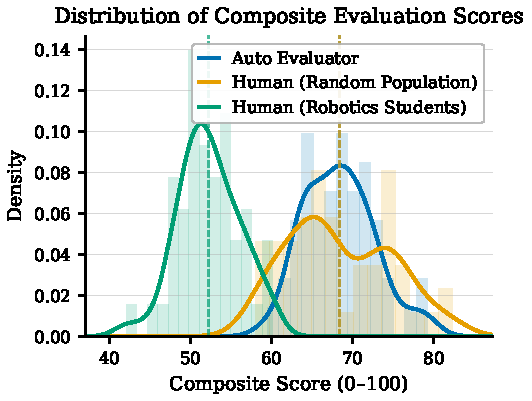
\includegraphics[width=\columnwidth]{assets/distribution_shift}
  \caption{Composite score distributions across evaluator groups.
           Dashed lines indicate group means.}
  \label{fig:distribution}
\end{figure}

%--------------------------------------------------
\section{Conclusion}

AsimovBM demonstrates that human-aligned perceptual evaluation of physical AI robotics
agents in social navigation can be automated without sacrificing evaluation
integrity.
A principled metric framework, combined with a client-server architecture that
simultaneously protects submitter intellectual property and prevents scenario
overfitting, provides a scalable alternative to per-configuration user studies.
Preliminary validation confirms alignment with lay-population judgment and
identifies an expert-calibration gap that motivates the collection of
domain-expert preference annotations to train axis-specific aggregation weights.
Future work will extend simulator telemetry to multi-agent pose streams, broaden
the scenario suite, and release AsimovBM as an open evaluation service with a
public leaderboard.

\newpage % @TODO remove, now just for show available space (2 page limit, exluding refs and appendix)

\bibliographystyle{IEEEtran}
\bibliography{bibliography}

%--------------------------------------------------
\appendices

\section{Sub-Indicator Specifications}
\label{app:metrics}

Each of the twelve sub-indicators produces a score in $[0,\,100]$ via the
threshold-anchored normalization of Eq.~\eqref{eq:norm}, with sign inversion
for lower-is-better quantities.
Threshold constants are stored in versioned scenario configuration, so
recalibration requires no formula change.
Let $\mathcal{E}$ denote valid behavioral episodes for a given tier and
$\mathcal{E}_s \subseteq \mathcal{E}$ successful ones, defined as episodes in
which the robot stops within the target stop band $[0.8,\,1.4]$\,m before the
timeout $T_{\max} = 120$\,s.
A macro-axis score is suppressed and reported as \textit{insufficient evidence}
when $|\mathcal{E}| < 3$ for that tier.

\subsection{Perceived Dexterity ($\mathcal{D}$)}

Perceived Dexterity quantifies how competently the robot executes the assigned
navigation task. All three sub-indicators are computed on successful episodes
only, except TSR which uses all valid episodes.

\textbf{Task Success Rate (TSR).}
The primary indicator of task competence, TSR is the fraction of valid
behavioral episodes in which the robot succeeds:
\begin{equation}
  \text{TSR} = \frac{|\mathcal{E}_s|}{|\mathcal{E}|}, \qquad
  R_\text{TSR} = 100 \cdot \text{TSR}.
\end{equation}
Good $\text{TSR} = 1.0$ (all episodes succeed), bad $\text{TSR} = 0.0$.

\textbf{Task Completion Time.}
A fast but correct completion is perceived as more dexterous.
The mean wall-clock duration over successful episodes,
\begin{equation}
  \bar{T} = \frac{1}{|\mathcal{E}_s|}\sum_{i \in \mathcal{E}_s} T_i,
\end{equation}
is normalized with $T_\text{good} = 0.35\,T_{\max}$ and $T_\text{bad} =
T_{\max}$, rewarding agents that complete the task well before the timeout.
Marked \textit{not applicable} when $|\mathcal{E}_s| = 0$.

\textbf{Path Efficiency ($\bar\eta$).}
Unnecessary detours signal hesitation or poor planning. Path efficiency is
the ratio of the collision-free shortest path $L^*$ to the actual traversed
length $L_i$, averaged over successful episodes:
\begin{equation}
  \bar{\eta} = \frac{1}{|\mathcal{E}_s|}
    \sum_{i \in \mathcal{E}_s} \frac{L^*}{\max(L_i,\,\varepsilon)}.
\end{equation}
Good $\bar{\eta} = 1.0$ (optimal path), bad $\bar{\eta} = 0.35$.

\subsection{Perceived Safety ($\mathcal{S}$)}

Perceived Safety captures whether the robot respects the personal space of
nearby humans, as defined by Hall's proxemics zones \tcite.
Let $d_j(t) = \|\mathbf{p}_r(t) - \mathbf{p}_{h,j}(t)\|_2$ be the
instantaneous Euclidean distance between the robot and the $j$-th human,
and $d(t) = \min_j d_j(t)$ the distance to the nearest person.

\textbf{Minimum Human-Robot Distance ($d_{\min}$).}
The closest the robot ever approaches any person during an episode:
$d_{\min} = \min_t d(t)$.
The good threshold is the personal-space boundary $d_\text{ps} = 1.2$\,m;
the bad threshold is the hard safety floor $d_\text{hard} = 0.45$\,m,
below which physical contact is imminent.

\textbf{Proxemic Intrusion Ratio ($\varrho$).}
Even brief intrusions are unpleasant; sustained ones are alarming.
This indicator measures the fraction of episode time the robot spends inside
personal space:
\begin{equation}
  \varrho = \frac{1}{T}\int_0^T
    \mathbf{1}\!\left[d(t) < d_\text{ps}\right] dt,
\end{equation}
with good $\varrho = 0$ (no intrusion) and bad $\varrho = 0.25$ (a quarter
of the episode spent inside personal space).

\textbf{Speed Near Humans ($\bar{v}_\text{near}$).}
A robot moving fast near people is perceived as unsafe regardless of
absolute distance. This indicator is the time-averaged speed while the robot
is within $d_\text{near} = 2.0$\,m of any human:
\begin{equation}
  \bar{v}_\text{near} =
    \frac{\displaystyle\int_0^T v(t)\,\mathbf{1}[d(t) < d_\text{near}]\,dt}
         {\displaystyle\int_0^T \mathbf{1}[d(t) < d_\text{near}]\,dt}.
\end{equation}
Good $\bar{v}_\text{near} \le 0.25$\,m/s, bad $\ge 1.0$\,m/s.
Marked \textit{not applicable} if the robot never enters the near-human zone.

\subsection{Perceived Social Awareness ($\mathcal{A}$)}

Perceived Social Awareness evaluates whether the robot interprets and responds
correctly to human social cues. All three indicators are driven by structured
\textit{come-here} task events, each specifying a target human identifier, the
instantaneous bearing error $\theta_e(t)$ between the robot's forward axis and
the target direction, and a fixed acknowledgement window $T_\text{ack} = 3$\,s.
This protocol avoids relying on visual gesture recognition, focusing instead
on observable navigational behavior.

\textbf{Gesture Response Success (GRS).}
This indicator checks whether the robot responds to the right person.
It is binary per episode: $\text{GRS}_i = 1$ if the robot begins moving toward
the designated target within $T_\text{ack}$ without first approaching a
non-target human, and $0$ otherwise.
\begin{equation}
  R_\text{GRS} = \frac{100}{|\mathcal{E}|}
    \sum_{i \in \mathcal{E}} \text{GRS}_i.
\end{equation}

\textbf{Acknowledgement Clarity (ACK).}
Before approaching, a socially aware robot should signal that it has
understood the request by facing the caller.
$\text{ACK}_i = 1$ if the robot's forward axis enters the cone
$|\theta_e(t)| \le 35^\circ$ within $T_\text{ack}$ and before locomotion
toward the target begins, and $0$ otherwise.
\begin{equation}
  R_\text{ACK} = \frac{100}{|\mathcal{E}|}
    \sum_{i \in \mathcal{E}} \text{ACK}_i.
\end{equation}

\textbf{Human-Aware Approach (HA).}
Approaching the target while disturbing bystanders is socially inappropriate.
This indicator jointly rewards target progress $\pi_i$ and bystander
clearance $\beta_i$:
\begin{equation}
  \text{HA}_i = 0.5\,\pi_i + 0.5\,\beta_i, \quad
  \pi_i = \operatorname{clip}\!\left(
    \frac{d_{0,i} - d_{f,i}}{d_{0,i}},\,0,\,1\right),
  \label{eq:ha}
\end{equation}
where $d_{0,i}$ and $d_{f,i}$ are the initial and final robot-to-target
distances, and $\beta_i$ is the fraction of episode time all bystanders
remain outside personal space.
Good $\text{HA} \ge 0.9$, bad $\text{HA} \le 0.4$.

\subsection{Impression ($\mathcal{I}$)}

Impression captures the overall quality and naturalness of robot motion,
independent of whether the task was completed. These indicators correlate with
how trustworthy and controlled the robot appears.

\textbf{Motion Smoothness (SPARC).}
Jerky motion is perceived as unpredictable and uncontrolled.
The SPARC index \tcite\ penalizes spectral power at high frequencies by
integrating the arc-length of the normalized speed spectrum
$\hat{V}(\omega) = V(\omega)/V(0)$, computed on the uniformly resampled
speed signal:
\begin{equation}
  \text{SPARC} = -\int_0^{\omega_c}
    \sqrt{\omega_c^{-2} +
      \left(\frac{d\hat{V}}{d\omega}\right)^{\!2}}\;d\omega.
  \label{eq:sparc}
\end{equation}
More negative values correspond to jerkier motion.
Good $\text{SPARC} = -2.0$, bad $\text{SPARC} = -6.0$.

\textbf{Stability / Controlledness (SC).}
Falls, collisions, and control failures strongly reduce the perceived
competence of a robot. This indicator aggregates instability events
$N_\text{inst}$, unintended contacts $N_\text{col}$, and invalid control
actions $N_\text{inv}$ into a single penalty:
\begin{equation}
  \text{SC} = 1 - \operatorname{clip}\!\left(
    \frac{N_\text{inst} + N_\text{col} + N_\text{inv}}{N_\text{bad}},
    \,0,\,1\right), \quad N_\text{bad} = 3.
\end{equation}
$R_\text{SC} = 100\cdot\text{SC}$; a robot with no adverse events scores
100, while three or more reduces the score to 0.

\textbf{Morphology-Task Fit (MTF).}
A robot that lacks required capabilities for the evaluation scenario will
perform poorly on every other indicator; this indicator makes that gap
explicit. It is the ratio of satisfied to required platform capabilities:
\begin{equation}
  \text{MTF} = \frac{|\mathcal{C}_\text{sat}|}{|\mathcal{C}_\text{req}|},
\end{equation}
where $|\mathcal{C}_\text{req}| = 5$ covers: approach locomotion,
forward-axis or sensor-facing metadata, an obstacle-distance sensor stream,
proprioception, and a controllable joint-target action mapping.
Good $\text{MTF} = 1.0$, bad $\text{MTF} \le 0.4$.

%--------------------------------------------------
\section{Per-Axis Score Distributions}
\label{app:figures}

Figures~\ref{fig:radar} and~\ref{fig:boxplot} complement Table~\ref{tab:metrics}
and Fig.~\ref{fig:distribution} in the main paper by breaking down scores
per axis and visualizing the full score distribution rather than just the mean.

\begin{figure}[h!]
  \centering
  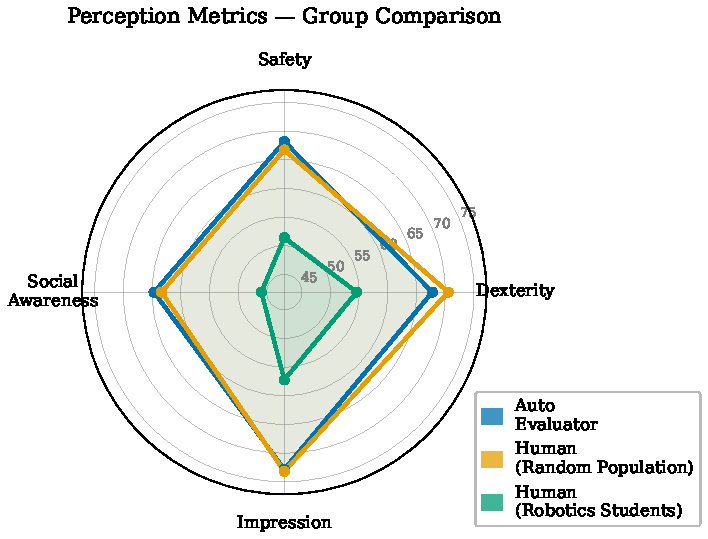
\includegraphics[width=\columnwidth]{assets/radar_plot}
  \caption{Mean per-axis scores for the three evaluator groups on a common
  $[0,\,100]$ scale. Each vertex represents one macro-axis; a larger enclosed
  area indicates higher overall perceived quality. The Auto Evaluator and Human
  (Random Population) profiles nearly overlap on all axes, while the expert
  panel (robotics students) contracts uniformly inward, with the sharpest
  drop on Social Awareness ($\Delta\bar{S} = 18.7$). This axis-specific gap
  indicates that equal-weight aggregation underweights gesture responsiveness
  relative to expert expectations.}
  \label{fig:radar}
\end{figure}

\begin{figure}[h!]
  \centering
  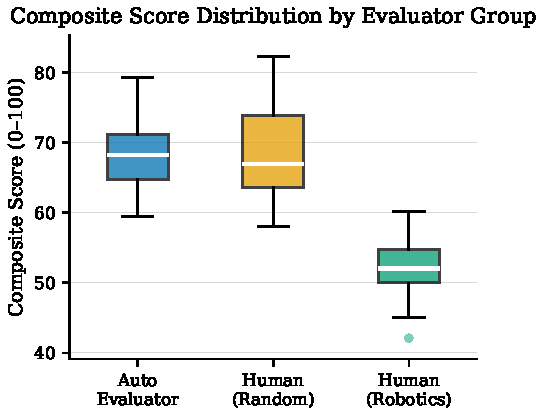
\includegraphics[width=\columnwidth]{assets/boxplot_global}
  \caption{Box plots of the composite score distribution for each evaluator
  group ($n = 50$ per group). The interquartile range and median confirm that
  the Auto Evaluator and Human (Random Population) groups agree not only in
  mean but also in spread, whereas the expert panel is both lower and less
  dispersed. The reduced variance of the expert group reflects a more
  consistent, domain-informed evaluation standard rather than random
  disagreement with lay raters.}
  \label{fig:boxplot}
\end{figure}

\end{document}
